\subsection{Problema a resolver}
El siguiente ejercicio consiste en hallar una manera de implementar un sistema proporcionado respetando una cota determinada de orden de complejidad. El problema se sitúa en un centro de distribución de correo que recibe paquetes todos los días cuyo destino final es la sede central de la empresa. Para el transporte de los mismos, éstos son cargados a camiones de igual capacidad. El encargado de logística, Pascual, tiene un sistema que utiliza desde hace años para agilizar la carga de los camiones asegurando el uso de una baja cantidad de los mismos para el envío de paquetes al final del día. Dicho sistema consiste en tomar los paquetes y ubicarlos en algún camión que ya tenga paquetes dentro, eligiendo entre éstos el que menos peso esté cargando hasta ese momento. Si el peso del paquete permite que éste sea cargado en ese camión, se lo ubica allí, sino, se lo incluye en un nuevo camión.\newline
El problema a resolver se basa en escribir un algoritmo que tome los pesos de los paquetes que hay que acomodar e indique cuántos camiones se van a utilizar y cuánto peso se cargará en cada uno de ellos al final del día considerando el sistema de Pascual. Para esto, se respeta el orden de llegada de los paquetes a medida que ingresan. \newline
Las consideraciones a tener en cuenta son que los camiones tienen todos la misma capacidad de carga, la cantidad disponible de los mismos alcanza para transportar todos los paquetes y que el peso de un paquete no supera la capacidad de carga de un camión. Del mismo modo, el tamaño de los paquetes no es tenido en cuenta, sino que se los identifica por su peso. Además, es importante aclarar que las cargas son valores enteros positivos.\newline
\newline
\textbf {Formatos de entrada y salida:}\newline
\newline
La entrada contiene varias instancias del problema. Cada instancia consta de una línea con el siguiente formato:

$$L\ n\ p_{1}\ p_{2}\ ...\ p_{n}$$


donde \textbf{$L$} es el límite de carga de los camiones, \textbf{$n$} es la cantidad de paquetes a acomodar y \textbf{$p_{1}$, ..., $p_{n}$} son los pesos de cada paquete en el orden en el que deben ser almacenados.\newline

La salida debe contener una línea por cada instancia de entrada, con el siguiente formato:

$$k\ c_{1}\ c_{2}\ ...\ c_{n}$$


donde \textbf{$k$} es la cantidad de camiones utilizados y \textbf{$c_{1}$, ..., $c_{k}$} es el peso que se cargó en cada uno de los \textbf{$k$} camiones al final del día.\newline

En lo que sigue, presentaremos dos ejemplos sobre el sistema impulsado por Pascual:
\begin{itemize}
\item {\large{\textbf{Ejemplo 1:}}}\newline

En este ejemplo, decidimos develar un caso en el que fuera agregado un paquete a un camión ya cargado. Por otro lado, quisimos contrarrestarlo insertando un paquete con una carga que superaba la capacidad del camión creado anteriormente. Por último, nos pareció importante mostrar un caso en el que al agregar un nuevo paquete, si bien un nuevo camión había sido creado, éste era colocado en el camión cuya carga fuera la menor.\newline

\textbf{Formato de entrada:}
$$100\ \ 5\ \ 20\ \ 40\ \ 80\ \ 15\ \ 100$$

\begin{figure}[H] %[h] Aqui [b] para button [t] para top
\begin{center}
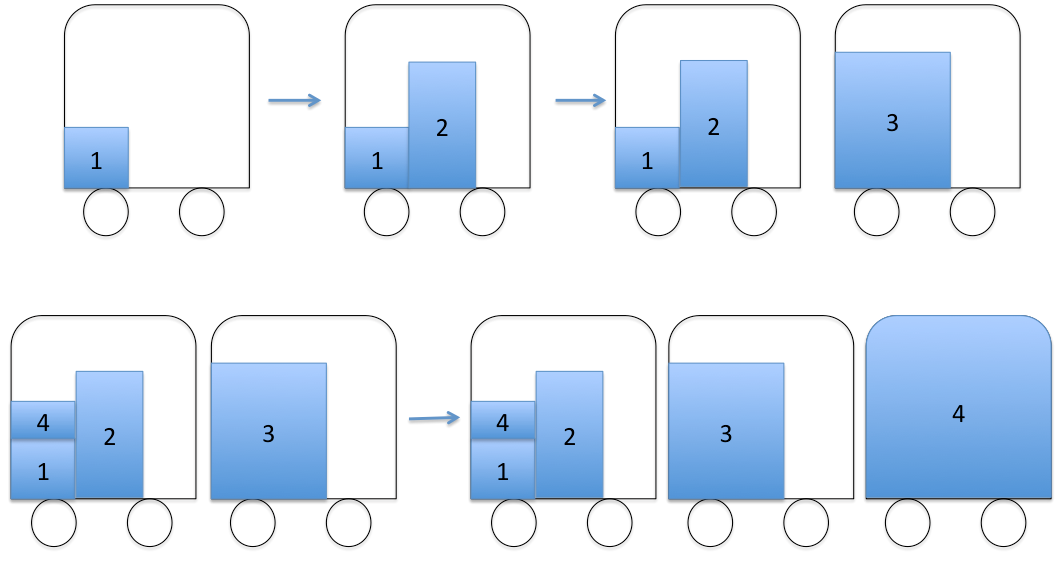
\includegraphics[width=320pt]{../imgs/ejemplo1.jpg}
\end{center}
\end{figure}

\textbf{Formato de salida:}
$$3\ \ 75\ \ 80\ \ 100$$


\item {\large{\textbf{Ejemplo 2:}}}\newline

En este ejemplo, quisimos mostrar lo que ocurría cuando cada paquete supera el 50\% de la carga disponible en un camión.\newline

\textbf{Formato de entrada:} 
$$150\ \ 3\ \ 80\ \ 75\ \ 82$$

\begin{figure}[H] %[h] Aqui [b] para button [t] para top
\begin{center}
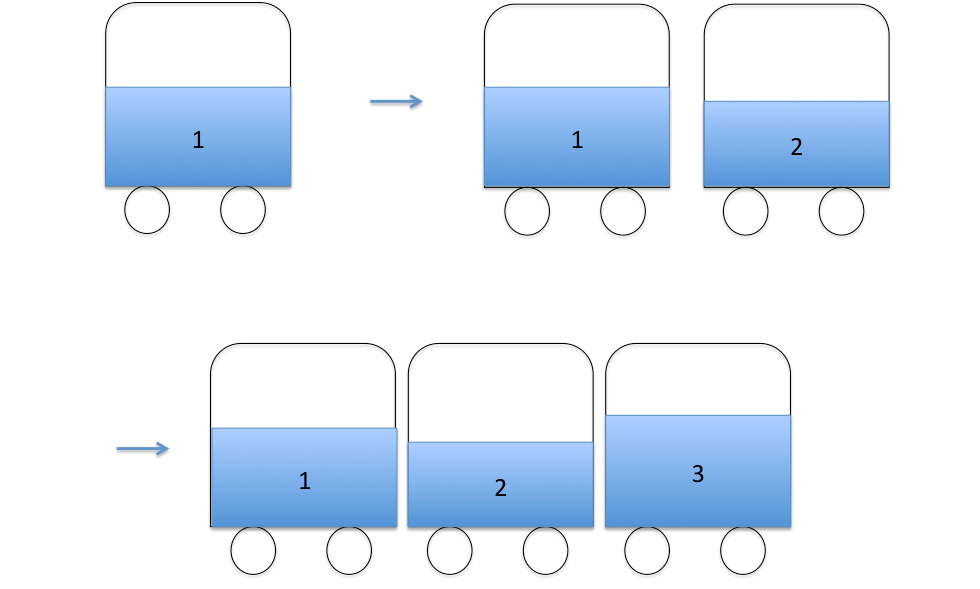
\includegraphics[width=300pt]{../imgs/ejemplo2.jpg}
\end{center}
\end{figure}

\textbf{Formato de salida:}
$$3\ \ 80\ \ 75\ \ 82$$


\end{itemize}
\subsection{Resolución coloquial}
Al analizar el problema a resolver, nos percatamos de que el algoritmo de Pascual corresponde a un $algoritmo\ goloso$. Dicho algoritmo consiste en la construcción de una solución seleccionando, en cada paso, la mejor alternativa sin considerar las implicancias de ésta.\newline Por otro lado, dicha técnica de diseño algorítmico resulta fácil de implementar, suele ser eficiente y permite construir soluciones razonables.\newline
\newline
En el caso del algoritmo de Pascual, el algoritmo goloso consiste en tomar cada instancia de la entrada y ubicarla en el lugar más conveniente en ese momento determinado. Esto significa que, dada la $i-ésima$ caja ingresada en un mismo día, ésta es ubicada en el camión que menor cargado se encuentra en ese momento. Para lograr esto, decidimos utilizar como estructura una cola de mínima prioridad.\newline
\newline
Una cola de prioridad consiste en una estructura de datos en la que sus elementos son atendidos según la prioridad que éstos tengan asociada. Dicha estructura se caracteriza por admitir inserciones de nuevos elementos y la consulta y eliminación del elemento de mínima prioridad.\newline
Las colas de prioridad suelen ser útiles para resolver algoritmos golosos ya que éstos suelen tener una iteración principal, y una de las tareas a realizar en cada una de dichas iteraciones es seleccionar un elemento de entre varios que minimiza un cierto criterio de optimalidad local.\newline
Para adaptar el problema de Pascual a la cola de prioridad, decidimos que cada elemento debía representar la carga correspondiente a un camión determinado en la instancia dada junto con el orden de creación del mismo.\newline
\newline
El pseudocódigo ideado para resolver el problema es el siguiente:\newline

\begin{algorithm}[H]
	\SetAlgoLined
	\caption{Algoritmo de Pascual}
	\KwIn{Entero limite, Paquetes $ps$}
	\KwOut{cantidadDeCamiones, listaDePesos}
	\lIf{$ps = \emptyset$}{\textbf{devolver} 0, $ListaVacia$}\\
	
	Camiones $ca \leftarrow$ \{Camion $cNuevo(0)\}$\\
	cantidadDeCamiones := 1\\
	\For{Paquete p $\in$ $ps$}{
		Camion $c$ := camionMenosCargado($ca$)\\
		\eIf{peso($p$)+capacidad($c$) $\leq$  limite}{
			capacidad($c$) $+=$ peso($p$)
		}{
			$ca \leftarrow$ Camion $cNuevo(0)$\\
			capacidad($cNuevo$) $=$ peso($p$)\\
			cantidadDeCamiones + 1;
		}
	}
	\textbf{devolver} cantidadDeCamiones, $ca$
\end{algorithm}

La función $cNuevo$ crea un nuevo camión cuya carga inicial es 0.\newline
\newline
La función $camionMenosCargado$ devuelve el camión menos cargado. Debido a que la estructura utilizada para almacenar los camiones provee dicha función, decidimos que no era necesario presentar el pseudocódigo de la misma.\newline

\subsection{Demostración de correctitud}
Para demostrar que nuestro algoritmo se corresponde con el algoritmo de Pascual, decidimos realizar una comparación, de forma paulatina, entre lo que define el algoritmo de Pascual y nuestro pseudocódigo.\newline
\newline
En primer lugar, podemos ver que una vez que ingresa un paquete, se analiza si éste entra en el camión menos cargado ya conteniendo algún paquete. En nuestro pseudocódigo, ésto corresponde a la línea 6.\newline
\newline
Luego, si el peso del paquete permite cargarlo en ese camión, se lo carga allí (línea 7). Caso contrario, se utiliza un nuevo camión para el paquete ingresado dándole como carga inicial la correspondiente a este último (líneas 9 y 10).\newline
\newline
Por último, podemos observar que la cantidad de camiones que se utilizan al final del día se acumula en la variable $cantidadDeCamiones$ y los pesos de camiones en orden se devuelven a través de $ca$.

\subsection{Complejidad del algoritmo}
Para el análisis de complejidad de nuestro algoritmo, llamamos $n$ a la cantidad de paquetes que ingresan como parámetro de entrada.\newline
\newline
Debido a que el algoritmo realizado consiste en una serie de operaciones básicas, comparaciones y asignaciones (cuyas complejidades son lineales), la complejidad del mismo puede determinarse a partir de los ciclos que éste realiza.\newline
\newline
Nuestro algoritmo fue implementado sobre una cola de mínima prioridad, luego, la extracción del camión menos cargado se realiza en $\mathcal{O}(log\ n)$\footnote{http://www.cplusplus.com/reference/queue/priority\_queue/} gracias a la función \textbf{pop()} provista por $stl$.\newline
\newline
Por otro lado, la inserción de un nuevo camión (\textbf{push()}) se realiza en $\mathcal{O}(log\ n)$ + $\mathcal{O}(1)$ = $\mathcal{O}(log\ n)$\footnotemark[1]. Esto se debe a que la cola de prioridad está implementada sobre un vector cuyo tamaño es equivalente a la cantidad de paquetes (correspondiente al peor caso, e.g. $Ejemplo\ 2$). Para lograr esto, debimos agregar un camión por cada paquete a la cola de prioridad y luego retirarlos uno por uno ($\mathcal{O}(n)$).\newline
\newline
El ciclo del código recorre los paquetes ingresados como parámetro. Debido a que los pasos que realiza el mismo constan de un condicional cuyos resultados consisten en asignaciones y operaciones simples, y la función $push()$ y $pop()$ ($\mathcal{O}(log\ n)$), la ejecución del mismo tiene un orden de $\mathcal{O}(n\ log\ n)$.\newline
\newline
Además del ciclo, el algoritmo llama a $top()$ ($\mathcal{O}(1)$\footnotemark[1]) y, luego, recorre la cola de prioridad en un ciclo para ordenar los camiones por orden de creación ($\mathcal{O}(n)$). El orden de estos pasos del algoritmo quedan envueltos por la complejidad del ciclo principal. Por lo tanto, pudimos comprobar que la complejidad temporal del algoritmo es $\mathcal{O}(n\ log\ n)$, siendo ésta estrictamente menor a $\mathcal{O}(n^2)$, que fue lo requerido por la cátedra.

\subsection{Código fuente}

\begin{figure}[H]
\begin{center}
\begin{verbatim}
Camion c = ca.top();
if ((ps[i]+c.second) <= limite){
    c.second += ps[i];
    ca.pop(); //elimina el camion menos cargado y en la siguiente linea lo vuelve a agregar
    ca.push(c);
}else{
    ca.push(make_pair(cantCamiones, ps[i])); //agrega un nuevo camion
    ++cantCamiones;
}
\end{verbatim}
\caption{Pasos que se realizan al ingresar un nuevo paquete.}
\end{center}
\end{figure}

\begin{figure}[H]
\begin{center}
\begin{verbatim}
while(!ca.empty()){
	Camion c = ca.top();
	vectorCamionesOrdenados[c.first] = c.second;
	ca.pop();
}
\end{verbatim}
\caption{Ordenamiento de los camiones con respecto al momento en el que fueron creados.}
\end{center}
\end{figure}

\subsection{Instancias posibles}
Para verificar la correctitud de nuestro programa, dispusimos variar estratégicamente las instancias de entrada al ejecutarlo.
\begin{itemize}
\item En primer lugar, ejecutamos el programa ingresando paquetes cuyos pesos fueran equivalentes al límite de los camiones. De este modo, nos aseguramos de no estar cometiendo errores de cotas. El resultado obtenido fue el esperado: una cantidad de camiones equivalente a la cantidad de paquetes ingresados cuyos pesos correspondían exactamente al de cada paquete.\newline
\textbf{Parámetro de entrada:}
\textbf{Parámetro de salida:}\newline
\item Por otra parte, probamos no ingresar ningún paquete para corroborar que la salida estuviera comprendida por una cantidad de camiones nula y una lista vacía.\newline
\textbf{Parámetro de entrada:}
\textbf{Parámetro de salida:}\newline
\item Por último, quisimos comprobar qué ocurría al tener dos camiones con la misma carga y que ésta fuera la menor. Pudimos constatar que el algoritmo elige el último camión cargado.\newline
\textbf{Parámetro de entrada:}
\textbf{Parámetro de salida:}\newline
\end{itemize}

De este modo, logramos abarcar los casos límite en los que la implementación pudiera haber encontrado algún problema. Dado que los resultados obtenidos fueron los esperados, determinamos que para todas las instancias válidas posibles de entrada nuestra implementación resulta correcta.

\subsection{Testing}

Para realizar las pruebas de complejidad, generamos instancias aleatorias de pesos de cajas alterando la cantidad de las mismas pero manteniendo estático el peso máximo de carga de los camiones. Estas instancias fueron generadas en $Matlab$ con la función \textin{randn} de forma tal a poder acotarlas por la capacidad de carga de los camiones. De este modo, logramos medir las pruebas de nuestro algoritmo para comprobar que la complejidad correspondiera con la mencionada anteriormente.

%\begin{figure}[H] %[h] Aqui [b] para button [t] para top
%\begin{center}
%\includegraphics[width=300pt]{../imgs/complejidadEj1.jpg}
%\end{center}
%\end{figure}
